% !TeX program = XeLaTeX
\documentclass[english,final]{scrartcl}

\usepackage{Sweave}

\usepackage{amssymb}
\usepackage{amsmath}
\usepackage{amsthm}
\usepackage{mathtools}

\usepackage{babel}

\usepackage[english=british]{csquotes}

\usepackage[backend=biber]{biblatex}
\addbibresource{biblio.bib}

\usepackage{fontspec}
\setmainfont{Linux Libertine O}
\setsansfont{Linux Biolinum O}

\usepackage{microtype}

\usepackage{siunitx}
\usepackage{booktabs}

\usepackage[colorlinks=true, linkcolor=blue, pdfborder={0 0 0}]{hyperref}

\usepackage{todonotes}
\usepackage[left]{showlabels}

\title{An analysis of the Old Faithful Geyser}
\subtitle{End of term report for the lecture\\Computational Statistics}
\author{Tim Adler}


\begin{document}
\Sconcordance{concordance:Geyser-Analysis.tex:Geyser-Analysis.Rnw:%
1 42 1}
\Sconcordance{concordance:Geyser-Analysis.tex:./setup.Rnw:ofs 43:%
1 7 1 1 6 1 1 1 16 1 1 1 10 1 1 1 7 1 1 1 6 1 1 1 5 4 1 1 31 3 1 1 20 2 %
1 1 16 2 1 1 20 2 1}
\Sconcordance{concordance:Geyser-Analysis.tex:Geyser-Analysis.Rnw:ofs 79:%
45}
\Sconcordance{concordance:Geyser-Analysis.tex:./introduction.Rnw:ofs 80:%
1 36 1}
\Sconcordance{concordance:Geyser-Analysis.tex:Geyser-Analysis.Rnw:ofs 117:%
47}
\Sconcordance{concordance:Geyser-Analysis.tex:./description.Rnw:ofs 118:%
1 10 1 1 4 1 2 1 3 1 2 6 1}
\Sconcordance{concordance:Geyser-Analysis.tex:Geyser-Analysis.Rnw:ofs 139:%
49}
\Sconcordance{concordance:Geyser-Analysis.tex:./fit.Rnw:ofs 140:%
1 7 1 1 16 2 1 1 22 1 1 1 9 1 1 1 42 1 1 1 15 1 1 1 29 4 1}
\Sconcordance{concordance:Geyser-Analysis.tex:Geyser-Analysis.Rnw:ofs 164:%
51}
\Sconcordance{concordance:Geyser-Analysis.tex:./model.Rnw:ofs 165:%
1 15 1 1 39 40 1}
\Sconcordance{concordance:Geyser-Analysis.tex:Geyser-Analysis.Rnw:ofs 222:%
53 4 1}
\Sconcordance{concordance:Geyser-Analysis.tex:./details.Rnw:ofs 227:%
1 44 1}
\Sconcordance{concordance:Geyser-Analysis.tex:Geyser-Analysis.Rnw:ofs 272:%
59}
\Sconcordance{concordance:Geyser-Analysis.tex:./recurrence.Rnw:ofs 273:%
1 10 1 2 2 1 4 1 2 10 1 2 2 1 4 1 2 2 1}
\Sconcordance{concordance:Geyser-Analysis.tex:Geyser-Analysis.Rnw:ofs 304:%
61}
\Sconcordance{concordance:Geyser-Analysis.tex:./density.Rnw:ofs 305:%
1 7 1 1 8 1 2 1 7 1 2 5 1 1 -19 4 0 1 4 6 0 1 19 4 1 1 -7 6 0 1 4 6 0 1 %
7 4 1}
\Sconcordance{concordance:Geyser-Analysis.tex:Geyser-Analysis.Rnw:ofs 358:%
63}
\Sconcordance{concordance:Geyser-Analysis.tex:./loss.Rnw:ofs 359:%
1 10 1 1 37 7 0 1 -33 6 1 1 4 1 2 11 1 1 11 3 1}
\Sconcordance{concordance:Geyser-Analysis.tex:Geyser-Analysis.Rnw:ofs 402:%
65}
\Sconcordance{concordance:Geyser-Analysis.tex:./implementation.Rnw:ofs 403:%
1 12 1 1 72 17 0 1 11 12 0 1 -79 4 1 1 98 20 0 1 -94 1 1}
\Sconcordance{concordance:Geyser-Analysis.tex:Geyser-Analysis.Rnw:ofs 475:%
67}
\Sconcordance{concordance:Geyser-Analysis.tex:./residue.Rnw:ofs 476:%
1 11 1 1 3 19 0 1 2 27 1 1 32 19 0 1 -28 31 1 1 4 3 2 7 1 1 12 8 0 1 -8 %
29 1 1 9 22 0 1 -5 48 1 1 4 1 2 1 10 1 2 2 1}
\Sconcordance{concordance:Geyser-Analysis.tex:Geyser-Analysis.Rnw:ofs 716:%
69 3 1}


\maketitle

%\listoftodos

%!Rnw root = Geyser-Analysis.Rnw
%!TeX root = Geyser-Analysis.Rnw

% concordance = no idea
% echo: Do not automatically print entered R code


% Load important libraries

% Setup variables

% Setup the geyser data structure and colors

% Loss function used

% Official Prediction Function

% Often used plots

% Fit function using the above defined loss function
% Internally uses the R optim method
% Furthermore a helper method that generates for a function fn(x,p) the 
% counterpart to minimize over.

% Computes the prediction error of our model using cross validation 
% and a special loss function.
% Think about adding error handling.

% Computes the average misses with this predictive function fn.
% Does not use predictive error, however. Perhaps change later

% If the predictive function predicts too short, how much longer does
% one have to wait on average?

% Creates a logistic function that has the two asymptotic levels as 
% parameters. The "velocity" and "location" of switch will be fixed.

%!Rnw root = Geyser-Analysis.Rnw
%!TeX root = Geyser-Analysis.Rnw

\section{Introduction}
\label{sec:introduction}

In this report we want to analyse the eruptions of the Old Faithful Geyser. This is a geyser at the Yellowstone National Park, which is known for its predictability, hence the name 'faithful'.

We will use the data used by Azzalini \& Bowman \cite{data}, which was measured from August 1, 1985 to August 15, 1985. The measurements were taken manually an example page of the notes can be found in \cite[2]{data}. 

The data set consists of two variables with overall 299 measurements. The types of the variables can be found in Table~\ref{tab:str}. For details please consult Appendix~\ref{sec:summary}. 

\begin{table}[htbp]
  \centering
  \begin{tabular}{rrrr}
    \toprule
    Variable & Name & Type & Comment\\
    \midrule
    1 & duration & numeric & Eruption duration in \si{\minute}\\
    2 & waiting & numeric & Waiting time since last \\
    & & & eruption in \si{\minute}\\
    \bottomrule
  \end{tabular}
  \caption{Structure of the geyser data set}
  \label{tab:str}
\end{table}

From the handwritten notes, we take that not all duration measurements were done thoroughly at night times only a classification was given (\enquote{short}, \enquote{medium}, \enquote{long}). Azzalini \& Bowman chose to translate those to \SI{2}{\minute}, \SI{3}{\minute} and \SI{4}{\minute}. In this analysis we use an implementation of the geyser data set which is given by the R framwork. Explicitely we use R version 3.2.3 (2015-12-10) on a x86-64-pc-linux-gnu machine and the geyser data set given by the \texttt{MASS} library (Version 7.3-45). In this implementation the translation is already incorporated. Figure~\ref{fig:cluster} shows lines at the appropriate durations. We chose to leave the data points in as they do not seem to influence the overall shape of the distribution that much. Additionally we do not want to describe the data set perfectly, but merely want a predictive model. 

As stated, in this analysis the main focus will lie on the task of finding a suitable predictive model for the waiting time until the next eruption. Before 1998 the waiting time was predicted using a linear model only taking the last eruption duration into account. According to Cook \& Weisberg \cite{pred} this function is given by
\begin{align}
\text{(next waiting time [min])} = 30 + 10 \cdot \text{(duration [min])}.
\label{eq:opred}
\end{align}
This graph can be found in Figure~\ref{fig:cluster} (left, violet line) and we can use it to determine the requirements for our predictive model. The central one is, that we do not so much want to describe the data set perfectly, but instead focus on minimzing the number of missed eruptions while on the same time trying to have a bearable additional waiting time if our model predicts \enquote{too short}.

To achieve this goal we will analyse the shape of the data and propose a proper framework for our model to translate our requirements into statistics.

%!Rnw root = Geyser-Analysis.Rnw
%!TeX root = Geyser-Analysis.Rnw

\section{Cluster detection}
\label{sec:data}

We have two variables, the (last) waiting time and the duration, which we want to use to predict the next waiting time. Figure~\ref{fig:cluster} shows that our data points cluster into three clouds. These clouds are color coded. We see that there is no obvious linear dependence between any of the two plotted relations. The official predictive function just seems to run parallel to the line through the two centers of duration plot clouds.
\vspace{-0.8cm}
\begin{figure}[htbp]
\setkeys{Gin}{width=0.45\textwidth}
\centering
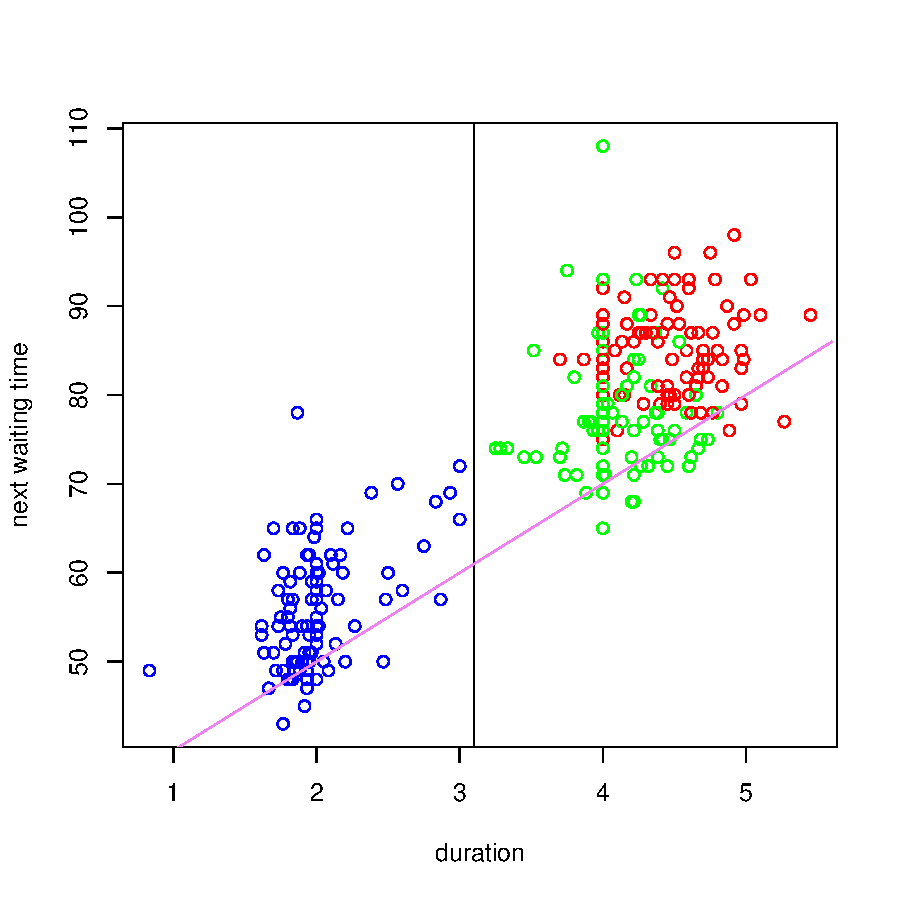
\includegraphics{Geyser-Analysis-dur_opred_plot}
\hspace{1cm}
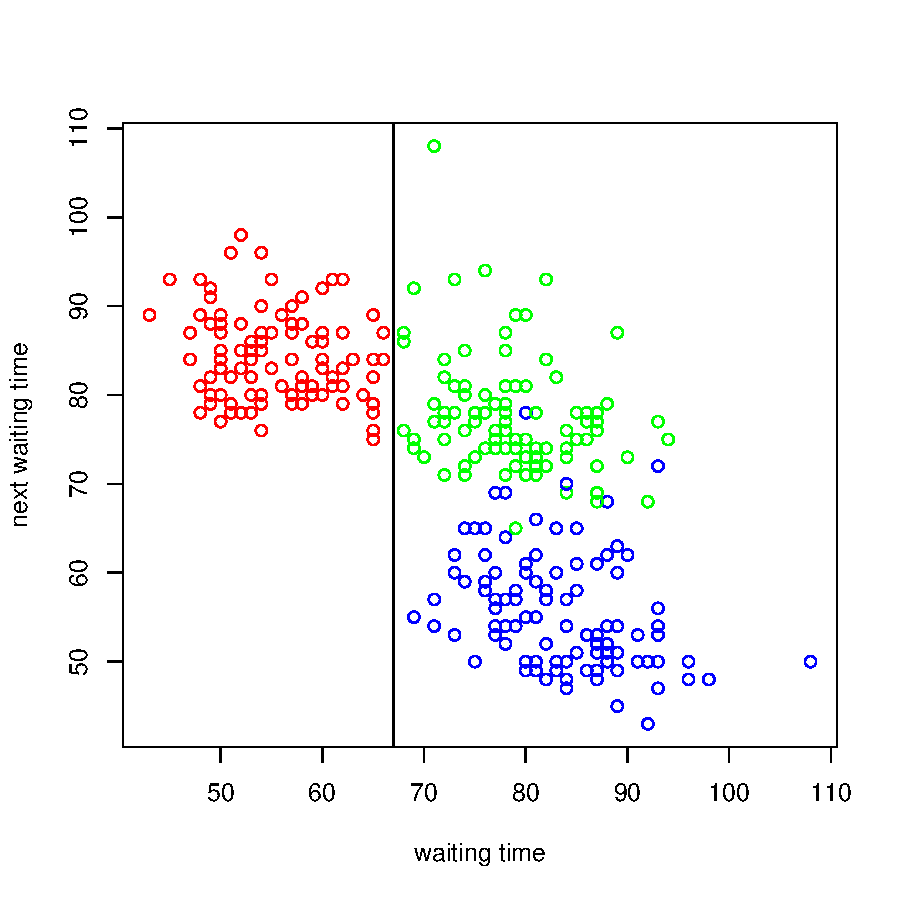
\includegraphics{Geyser-Analysis-wait_plot}
\caption{Color coded marginal scatter plots with separators and park model.}
\label{fig:cluster}
\end{figure}

We separate the three clouds by the two vertical lines depicted in Figure~\ref{fig:cluster}. The duration separator is at 3.1 and the wating time separator is at 67. This is not a perfect seperation as some points of the blue grouping mix with the green grouping and vice versa. Also the exact location of the waiting time split is up to some arbitration. It turns out that this is not a problem, because only one model (and not the best one) uses this separation. There are no other clusters in this data set as can be seen in Figure~\ref{fig:density} in Appendix~\ref{sec:details} on page~\pageref{fig:density}.

Azzalini \& Bowman \cite{data} state a rough physical model for the evolution of the waiting time, which involves a periodic process with period 2. It does not seem likely to us that we have such a simple periodicity. The details can be found in Appendix~\ref{sec:recurrence}.

%!Rnw root = Geyser-Analysis.Rnw
%!TeX root = Geyser-Analysis.Rnw

% This file contains the fits of the four chosen models.

% 0.) Fit waiting distribution
% Fit a mixed normal distribution to the distribution of the
% waiting times (no regard to duration)

% Fit a mixed normal distribution to the above distribution. The weight
% now depends logistically on the duration.

% 1.) Fit Logistic interpolation

% 2.) Fit PLM (dur)

% 3.) Fit LM (dur+wait)

% 4.) Fit PLM (dur+wait)

% 5.) Compute Predictive Error (Cross Validation)
% !!! Evaluation is normally turned of, since it takes quite long. The
% !!! values are buffered (manually) in the variables in setup.Rnw
% !!! Last one alone took 45 min to compile.

%!Rnw root = Geyser-Analysis.Rnw
%!TeX root = Geyser-Analysis.Rnw
\section{Model Framework}

We had a look at four different models and compared their predictions to the official predictive model. For that we set up our own loss function as depicted in Figure~\ref{fig:loss} on page~\pageref{fig:loss}. The procedure to determine its parameter can be found in Appendix~\ref{sec:loss}. The four investigated models are:
\vspace{-0.5ex}
\begin{enumerate}
\setlength{\itemsep}{-0.5ex}
\item A logistical interpolation of the two clouds shown in Figure~\ref{fig:cluster} (left).
\item A piecewise linear regression separating the two duration clouds.
\item A linear regression taking the duration as well as the last waiting time into account.
\item A piecewise linear regression separating the three clouds in Figure~\ref{fig:cluster} taking the duration and the last waiting time into account.
\end{enumerate}

The exact implementations of the fitting algorithm and the models is described in Appendix~\ref{sec:implementation} and~\ref{sec:models}. We also used cross validation to determine the predcitive total loss of our models (c.f.\ Appendix~\ref{sec:implementation}). The results can be found in Table~\ref{tab:model_summary}. The residuals of each of the models together with their fitted parameters are stated in Appendix~\ref{sec:models}.

\begin{table}[htbp]
\centering
\sisetup{
  table-number-alignment = right,
  table-figures-integer = 4,
  table-figures-decimal = 2
}
\begin{tabular}
{r
S
S[table-auto-round]
S[table-auto-round]
S[table-auto-round]
S[table-auto-round]}
\toprule
& {Number of}& {Fitted} & {Predictive} & {Average} & {Average}\\
& {Param} & {Total Loss} & {Total Loss} & {Misses} & {Additional Wait}\\
& & & & {[\%]} & {[\si{\minute}]}\\
\midrule
Official & 2&4053.83& 4053.83 & 10.07&8.74564675746269\\
\midrule
Logistic Interpolation & 2 
  & 3445.19879915965 & 3488.03
  & 2.3489932885906 & 10.4680371105143\\
Pw Linear (dur) & 4 
  & 3431.46347406616 & 3548.98 & 3.02013422818792 
  & 10.0984895296407\\
Linear (dur+wait) & 3
  & 3533.46797628286 & 3873.74
  & 1.67785234899329 & 11.0869214207606\\
Pw Linear (dur+wait) & 9
  & 3184.26955186659 & 3354.9
  & 3.35570469798658 & 9.07732483287011\\
\bottomrule
\end{tabular}
\caption{Summary of the models}
\label{tab:model_summary}
\end{table}

\section{Conclusion}
In conclusion we see that differentiating between the different clusters strongly improves the models. Model 3 (the only one not using clusters) can be discarded immediately. Its predictive total loss is by far the worst, because of the lack of used structure. The last model has the best predictive loss and smallest average waiting time, however the average miss ratio is slightly worse than for the other two. Together with the high amount of parameters necessary I would advise against its use. Perhaps in a later analysis one could consider a piecewise linear model with duration and waiting time as predictors, but only taking the duration separation into account. This would reduce the number of parameters to 6. As a standard choice I would recommend Model 1 as it has the best predictive behaviour, if the additional waiting time is of grave importance one could consider switching to Model 2, although the improvement is nigh negligible.

\newpage

\appendix

%!Rnw root = Geyser-Analysis.Rnw
%!TeX root = Geyser-Analysis.Rnw

\section{Descriptive Statistics}
\label{sec:details}

\subsection{Extended summary}
\label{sec:summary}

In the following section we describe the geyser data set in more detail. In addtion to what was mentioned in Section~\ref{sec:introduction}, we want to add that we have to keep in mind that waiting time $i$ of the data set denotes the waiting time \emph{before} eruption $i$ occured. Thus waiting time $i$ incorporates duration $i-1$. We could separate the two. However, as can be seen in Table~\ref{tab:summary}, the duration is much smaller than the waiting time such that the effect on the prediction would be negligible.

\begin{table}[htbp]
\centering
\sisetup{
  table-number-alignment = right,
  table-figures-integer = 3,
  table-figures-decimal = 2
}
\begin{tabular}{r
S[table-auto-round]
S[table-auto-round]}
\toprule
& {waiting} & {duration}\\
& {[\si{\minute}]} & {[\si{\minute}]}\\
\midrule
Min & 43 & 0.8333333\\
1st Quantile & 59 & 2\\
Median & 76 & 4\\
Mean & 72.314381270903 & 3.46081382508361\\
3rd Quantile & 83 & 4.3833333\\
Max & 108 & 5.45\\
\bottomrule
\end{tabular}
\caption{Summary of the geyser data set}
\label{tab:summary}
\end{table}

In Figure~\ref{fig:density} we see a 3 dimensional scatter plot of the next waiting time over waiting time and duration. A density estimation has been added and we see, that there are three clouds visible. These correspond exactly to the coloring in Figure~\ref{fig:cluster}.

\begin{figure}[htbp]
\centering
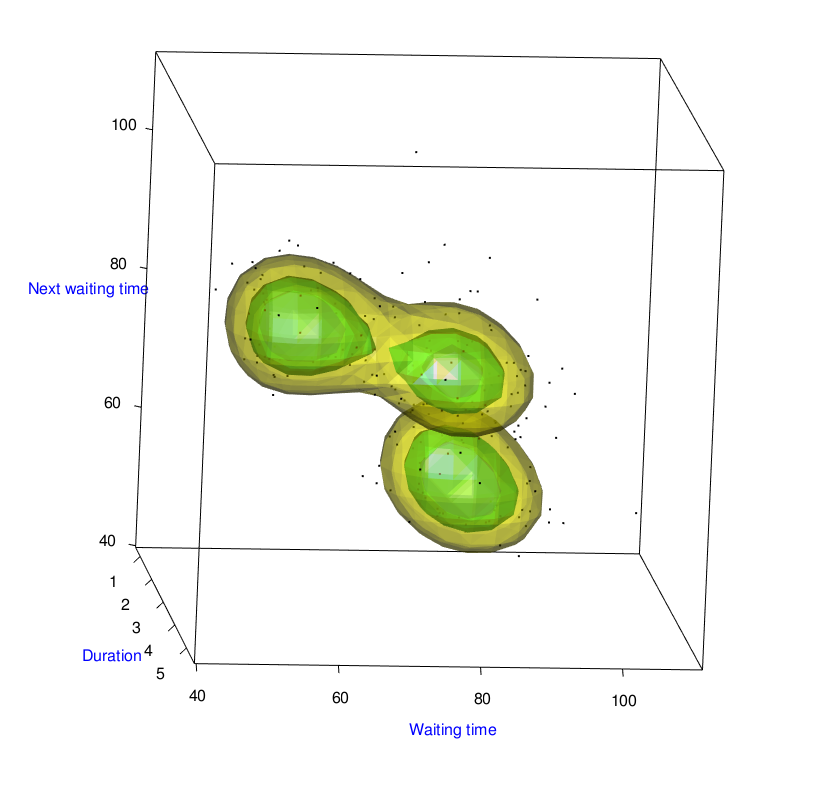
\includegraphics[width=0.65\textwidth]{density.png}
\caption{Three dimensional scatter plot with estimated density. We find three clusters corresponding to the clusters marked in Figure~\ref{fig:cluster}}
\label{fig:density}
\end{figure}

%!Rnw root = Geyser-Analysis.Rnw
%!TeX root = Geyser-Analysis.Rnw

\subsection{Periodicity and Recurrence Plots}
\label{sec:recurrence}

As Azzalini \& Bowman state in \cite{data}, they suspect a rough physical model underlying the eruption pattern of the geyser. One prediction of this model were that the waiting time would have a period of 2, i.e.\ the waiting time would alternate between \enquote{long} and \enquote{short}. Figure~\ref{fig:ts} (left) seems to back this idea. 

\begin{figure}[htbp]
\setkeys{Gin}{width=0.45\textwidth}
\centering
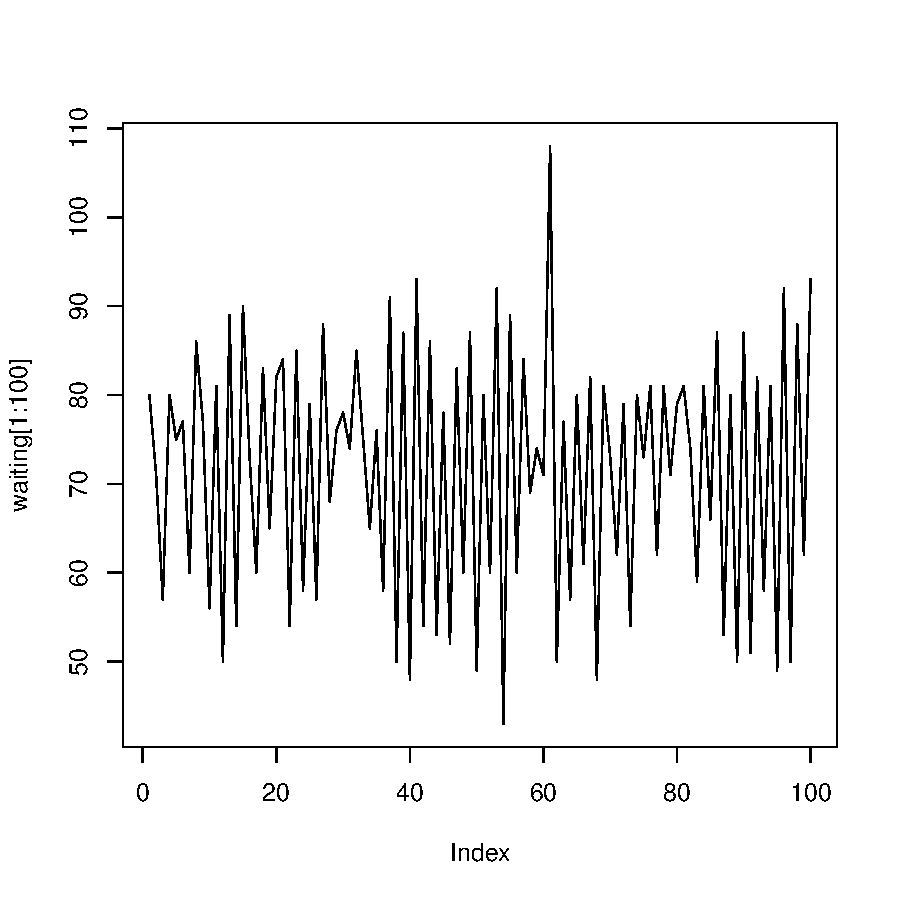
\includegraphics{Geyser-Analysis-plot_wait_period}
\hspace{1cm}
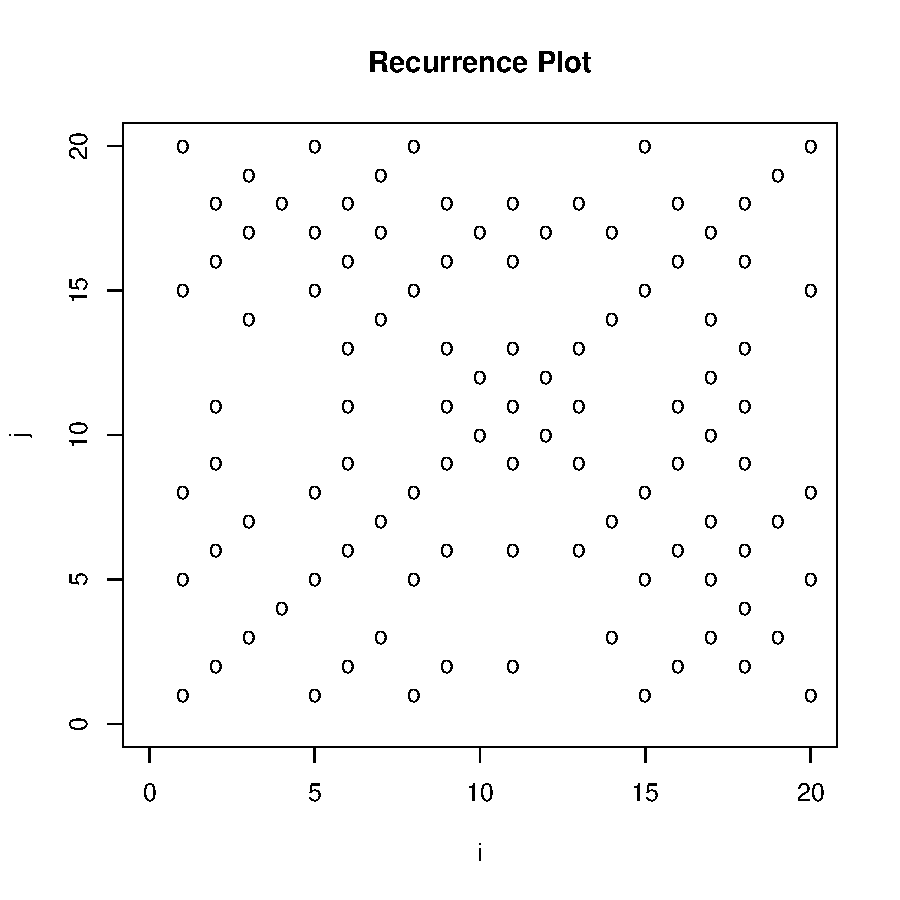
\includegraphics{Geyser-Analysis-rec_waiting_plot}
\caption{Left: Extract of the waiting time time series. Right: Extract of the waiting time recurrence plot.}
\label{fig:ts}
\end{figure}

To investigate the periodicity of our data set further, we used a recurrence plot as introduced in \cite{recurrence}. Recurrence plots give us a mark at coordinate $(i,j)$ whenever the waiting time at point $i$ is \emph{sufficiently} close to that of $j$. In our case we compared three consecutive data points starting at $i$ with their counterpart at $j$ and wanted them to be closer together than one standard deviation (13.89), which is a rather lenient restriction.

We see in Figure~\ref{fig:ts} (right), that we have basically no recurrences at $(i,i+2)$, which we would expect, if we had a periodicity of two. There are quite a few other recurrences, which is not surprising as our closeness constraint is rather lax, however it seems that all in all the period is either too long or too complex to be taken into account in the further analysis.

\begin{figure}[htbp]
\setkeys{Gin}{width=0.45\textwidth}
\centering
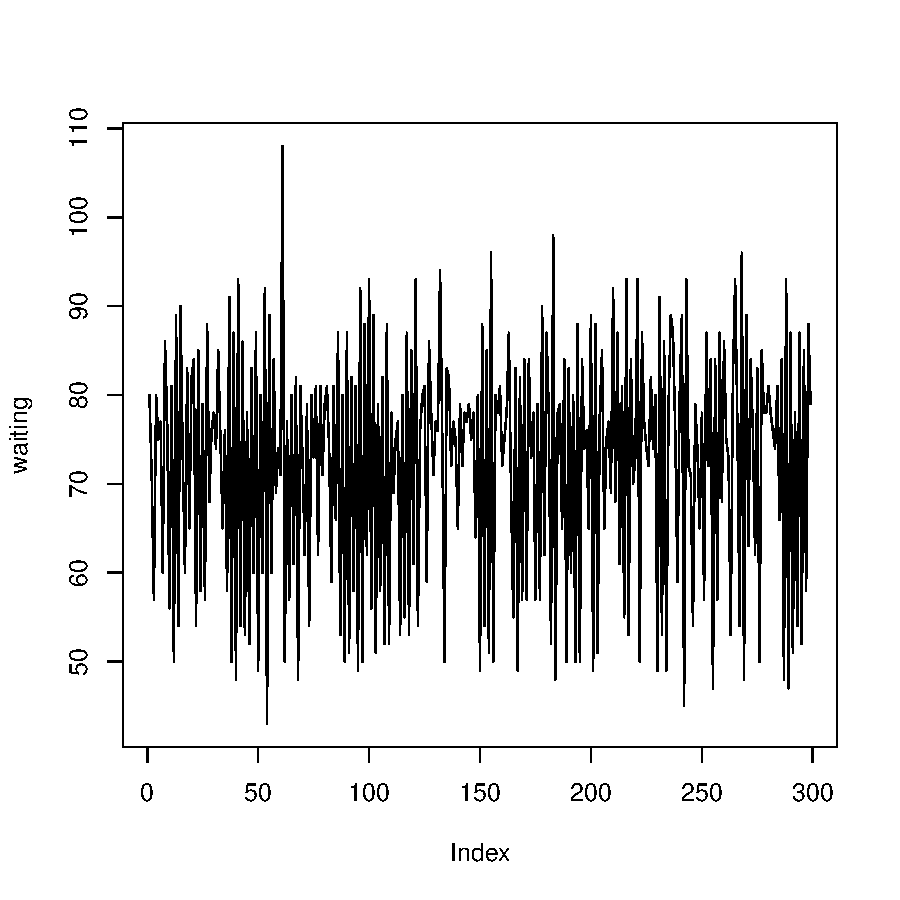
\includegraphics{Geyser-Analysis-plot_wait_period2}
\hspace{1cm}
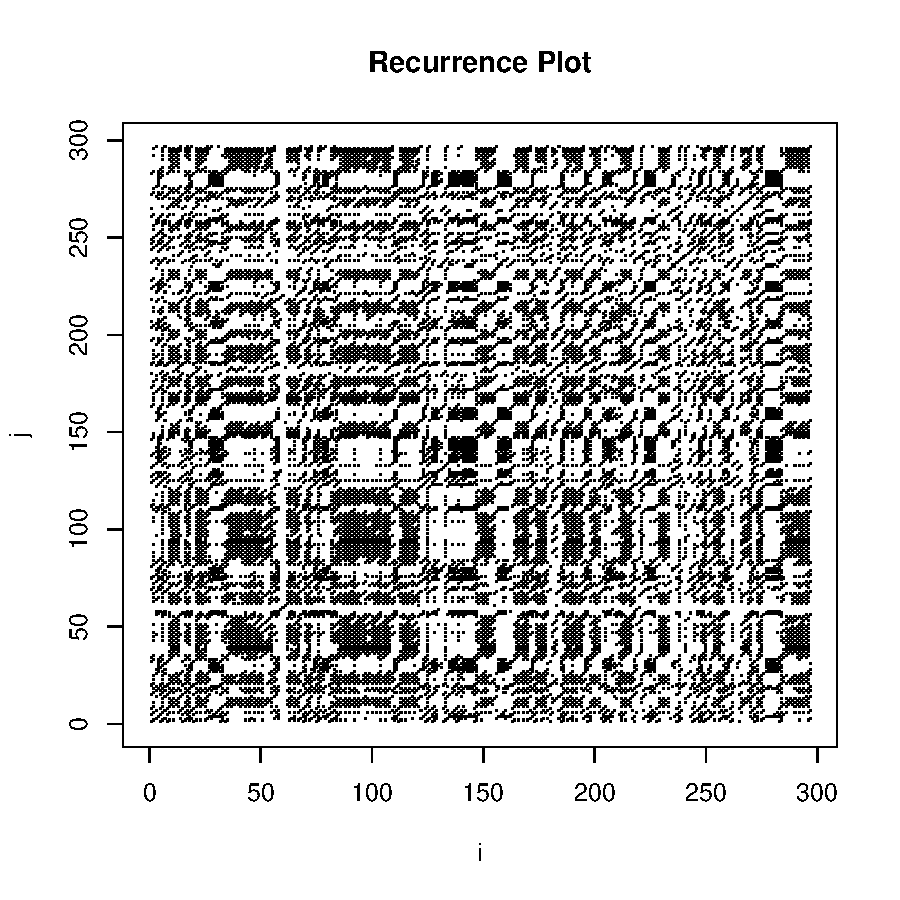
\includegraphics{Geyser-Analysis-rec_waiting_plot2}
\caption{Left: Full waiting time time series. Right: Full waiting time recurrence plot.}
\label{fig:ts2}
\end{figure}

\subsection{Nonparametric and parametric density estimation}
\label{sec:density}

Since we want to predict the waiting time it is interesting how the waiting time is distributed overall. For that we utilised a density estimation. We used the \texttt{density} method of R together with the Sheather-Jones-Algorithm(c.f.~\cite{sj}) for Bandwidth gauging. The problem is that we wanted to estimate the overall shape without averaging out important structure. To take this into account we also had a look at estimated densities with a far smaller bandwidth and found that the estimated bandwidth is appropriate for our purpose. The result of the estimation can be found in Figure~\ref{fig:wait} (left, black curve). 

\begin{figure}[htbp]
\setkeys{Gin}{width=0.45\textwidth}
\centering
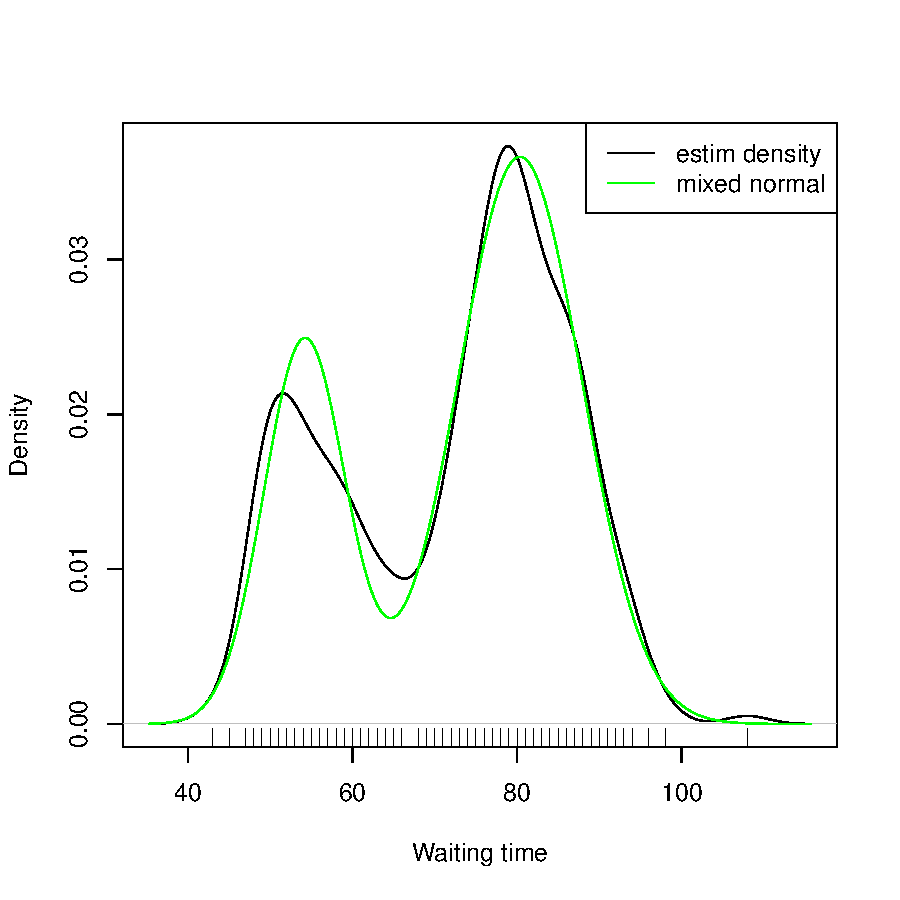
\includegraphics{Geyser-Analysis-dens_estim}
\hspace{1cm}
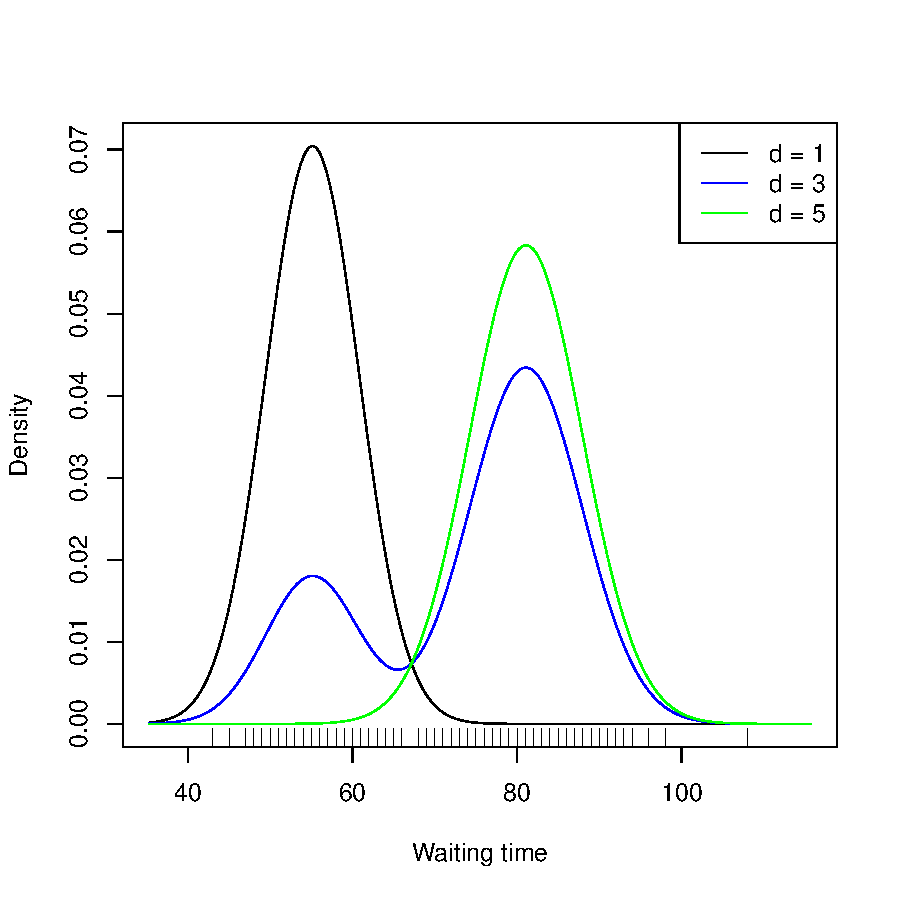
\includegraphics{Geyser-Analysis-plot_mn_density2}
\caption{Density estimation of the Waiting time. Left: Duration independet. Right: Duration dependent.}
\label{fig:wait}
\end{figure}

We observe that the distribution is strongly bimodal and from the form we deduce that it should be well described by a mixed normal distribution. We did this approximation (blue curve in Figure~\ref{fig:wait} left) following the procedure described in \cite{density}. Our density candidate is given by

\begin{Schunk}
\begin{Sinput}
> dwait1 <- function(x,p) {
+   p[1]*dnorm(x, mean = p[2], sd = p[3]) +
+     (1-p[1])*dnorm(x, mean = p[4], sd = p[5])
+ }
> dwait1.min <- function(x, p) {
+   e <- dwait1(x,p)
+   if(any(e <= 0)) Inf else -sum(log(e))
+ }
\end{Sinput}
\end{Schunk}

We minimize \texttt{dwait1.min} using the built in minimizer \texttt{optim} of R. As we see in Figure~\ref{fig:wait} the blue curve is in rather good agreement with the estimated density. However, the left peak is a little off and the overall form of it differs from the nonparametric density.

To remedy this shortcoming we want to introduce (as described in \cite{density}) another parameter and take the duration into account. Looking at Figure~\ref{fig:cluster}, it is clear that the duration has a strong impact on the distribution of the waiting time, so it seems sensible to make the density duration dependent. For this we make the \enquote{mixing coefficent} duration dependent. Since this coefficient has to vary between 0 and 1 it is natural to assume a logistic relation to the duration. Implemented this takes the following form:

\begin{Schunk}
\begin{Sinput}
> dwait2 <- function(x,y,p) {
+   q <- exp(p[1] + p[2]*y)
+   q <- q/(1+q)
+   q*dnorm(x, mean = p[3], sd = p[4]) +
+     (1-q)*dnorm(x, mean= p[5], sd = p[6])
+ }
> dwait2.min <- function(x,y,p){
+   e <- dwait2(x,y,p)
+   if(any(e <= 0)) Inf else -sum(log(e))
+ }
\end{Sinput}
\end{Schunk}

Analogously to \texttt{dwait1} we minimized it using \texttt{optim}. We see that for the one additional parameter we get a minimum of 985.32 as compared to 1154.24 for \texttt{dwait1}. This is a remarkable improvement. In Figure~\ref{fig:wait} (right) the waiting time distribution is plotted at different durations. We see that if the duration time is either very high or very low, the bimodal distribution degenerates to a common normal distribution.

Since we now have this very managable duration dependent distribution, we can easily obtain a predictive model for the waiting time. We simply compute the expectation value of the distribution, which depends logistically on the duration. This is the very first predictive model we use as can be seen in Appendix~\ref{sec:models}.


%!Rnw root = Geyser-Analysis.Rnw
%!TeX root = Geyser-Analysis.Rnw

\section{The loss function}
\label{sec:loss}

In order to achieve our goal to find a suitable model to predict the waiting time of the faithful geyser, we need to work with an appropriate loss function. 

The standard loss function (i.e.\ minimizing over the quadratic error) does not seem to be a permissible candidate. A good model should take into account that it is far less annoying for a visitor to wait a couple of minutes at the geyser before the eruption starts than being a few minutes too late. Because of the symmetry of the quadratic error, it cannot distinguish between 'being too early' and 'being late'. 

Thus we will use the following loss function
\begin{Schunk}
\begin{Sinput}
> loss <- function(x, q){
+   x[x < 0] <- q
+   x
+ }
\end{Sinput}
\end{Schunk}
with parameter $q$.

As can be be seen in Figure~\ref{fig:loss}, the function attributes a constant high loss, if the prediction is too long and a linear gain of loss, if the predicted waiting time is shorter than the actual waiting time. This fullfills the requirement that a missed eruption weighs heavier than additional waiting time.

\begin{figure}[htbp]
\setkeys{Gin}{width=0.45\textwidth}
\centering
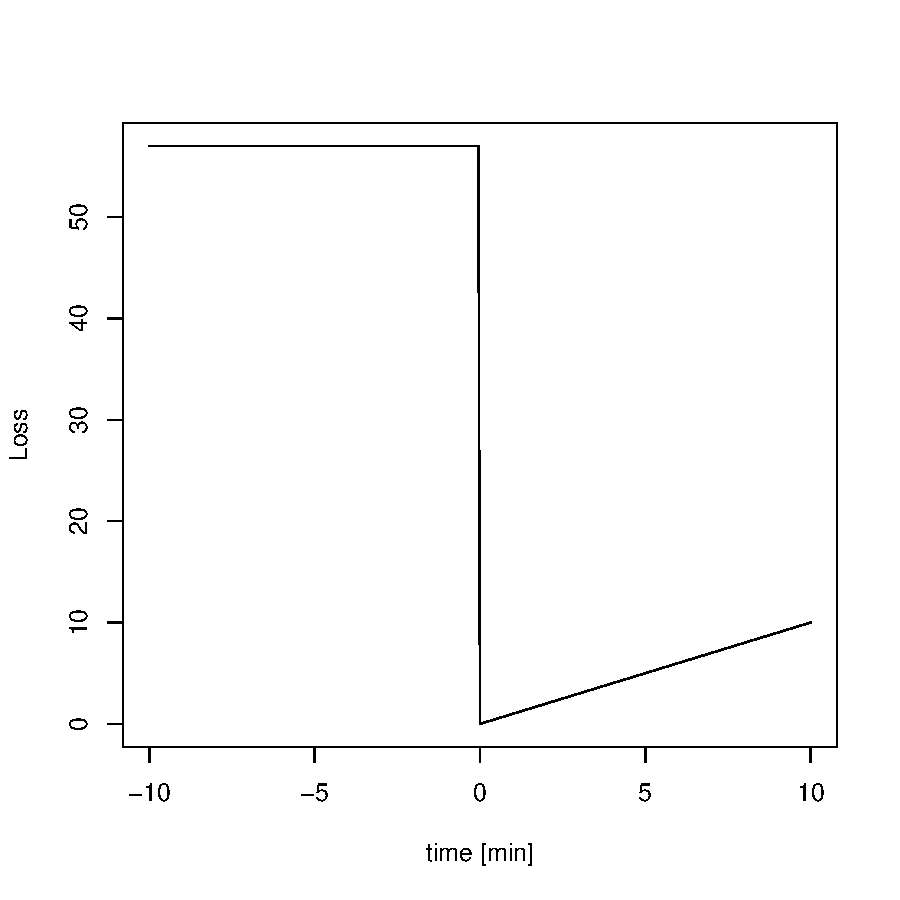
\includegraphics{Geyser-Analysis-plot_loss}
\caption{Proposed loss function. Positive time corresponds to a shorter predicted waiting time than the actual waiting time.}
\label{fig:loss}
\end{figure}

The last necessary step is to determine the parameter of this function. At first glance it seems that there are two: The slope of the linear part and the intercept of the constant part. However scaling the function by a (postive) factor does not change the result of a minimization. So we are free to fix the slope to 1 and are left with only the intercept as parameter. In order to determine it, we use the official predictive function of the National Park (as mentioned in~\cite{pred}, c.f.\ Equation~\eqref{eq:opred} on page~\pageref{eq:opred}).

The procedure to determine our parameter $q$ now consists in the following idea: If we have the right $q$ and we fit a linear model using this loss function we want to get the official park function. This idea is sensible, as we can assume that there certainly was a bit of optimization (and rounding) involved in the determination of the park function and we thus can make sure that we roughly apply the same error margin as the park.

Therefore the (manually) applied algorithm consists in systematically choosing different values for $q$ and then fitting a linear model. Aftewards we check the intercept and slope. If both are \enquote{close enough} to 30 respectively 10, we found our parameter.

The fitting procedure used is described in Appendix~\ref{sec:implementation}. To make sure that we end up in the right local minimum, we choose 30 and 10 as the inital parameters for the fit of the linear model.


For $q = 57$ we yield fit parameters 29.95 and 9.02. We also see that the models are rather robust with respect to small changes in $q$. So $q = 57$ seems an acceptable choice. $q$ lies in a sensible region, too. A short sanity check: With that choice it is as bad to miss an eruption (and thus having to wait another average waiting time) as it is bad to have to wait another average waiting time (c.f.\ Table~\ref{tab:summary} on page~\pageref{tab:summary}) to the next eruption after the predictive model said it should be. This sounds reasonable.

With this we get the total loss of the predictive park function as 4053.83. This is from now on our margin to top for alternative models.

%!Rnw root = Geyser-Analysis.Rnw
%!TeX root = Geyser-Analysis.Rnw

\section{The fit and cross validation routine}
\label{sec:implementation}

If we are given predictors $x \coloneqq (x_i)_{i=1,\dots,n}$ and regressors $ y \coloneqq (y_i)_{i=1,\dots,n}$ and a model function $f_p$ with parameter(s) $p$. We want to choose the parameter(s) in a manner such that the overall loss of the prediction is minimal. That means we want to solve the minimisation problem
\[
\min_p g(p, x, y) \coloneqq \min_p \sum_{i=1}^n \operatorname{loss}(y_i - f_p(x_i)).
\]

In R this problem takes the following form: The method \texttt{genmin} takes the function $f_p$ and generates the function $g$ we want to minimize over. The method \texttt{lossfit} takes $f_p$ internally generates $g$ and then uses the R intern minimizer \texttt{optim} with the Nelder-Mead-Algorithm (c.f.~\cite{nm}) and initial parameter $p_0$ to estimate the parameter $p$. In code this looks as follows:

\begin{Schunk}
\begin{Sinput}
> # takes a function fn(x,p) and generates a function to minimize over.
> genmin <- function(fn, l = loss, bound = q) {
+   function(p,x,y) {
+     result <- 0
+     if(is.atomic(x)) {
+       for(i in 1:length(y)) {
+         result <- result + l(y[i] - fn(x[i], p), bound)
+       }
+     } else {
+       for(i in 1:length(y)) {
+         result <- result + l(y[i] - fn(x[i,], p), bound)
+       }
+     }
+     #sum(loss(y - fn(x,p), bound))
+     result
+   }
+ }
> # fitting/minimization taking place here
> # p0: initial parameter
> # x: all predictors (as data.frame)
> # y: the (1d) regressor
> # l: custom loss function
> # bound: bound of the loss function
> lossfit <- function(p0, fn, x, y, l = loss, bound = q){
+   fn.min <- genmin(fn, l = l, bound = bound)
+   optim(p0, fn.min, x = x, y = y)
+ }
\end{Sinput}
\end{Schunk}

As any numerical optimizer/minimizer, \texttt{optim} only finds local minima and therefore $p$ critically depends on the chosen $p_0$. The method applied to finding $p_0$ is given for each model separately in Appendix~\ref{sec:models}.

The cross validation routine iterates over the regressor predictor pairs, always leaving one out and computing the fit completely analogously to the fit method. Afterwards it uses the parameter to compute the loss of the left out data point. These losses are added up and returned. The code is as follows:

\begin{Schunk}
\begin{Sinput}
> # p0: initial parameter
> # x: all predictors (as data.frame)
> # y: the (1d) regressor
> # l: custom loss function
> # bound: bound of the loss function
> losscv <- function(p0, fn, x, y, l = loss, bound = q) {
+   fn.min <- genmin(fn, l = l, bound = bound)
+   result <- list(value = 0, warn = c())
+   for(i in 1:length(y)) {
+     o <- optim(p0, fn.min, x = x[-i,], y = y[-i])
+     if (o$convergence != 0) {
+       result$warn <- append(result$warn, values = i)
+     } 
+     result$value <- result$value + fn.min(o$par, x[i,], y[i])
+   }
+   result
+ }
\end{Sinput}
\end{Schunk}

Again we have the problem of having to choose an initial parameter $p_0$. Therefore we reused the initial parameters of the fit routine.

%!Rnw root = Geyser-Analysis.Rnw
%!TeX root = Geyser-Analysis.Rnw

\section{Model implementation and residues}
\label{sec:models}

In the following we show the implementation of each of the used models, the residues after the fit, the strategy for obtaining the initial parameters and the values of the estimated parameters.

\subsection{Logistic interpolation with regressor: duration}

This model is just a standard implementation of a logistic function interpolating between two plateaus. The parameters of the exponential function, which determine the transition region and speed are fixed and taken from the fit of the duration dependent waiting time distribution (c.f.\ Appendix~\ref{sec:density}). Thus the implementation takes the form:

\begin{Schunk}
\begin{Soutput}
A single object matching ‘lg1.wait’ was found
It was found in the following places
  .GlobalEnv
with value

function(x,p) {
    if(is.atomic(x)) {
      d <- x
    } else {
      d <- x$d
    }
    q <- exp(l[1] + l[2]*d)
    q <- q/(1+q)
    q*p[1] + (1-q)*p[2]
  }
<environment: 0x26191a8>
\end{Soutput}
\end{Schunk}

As initial parameters for the plateaus we chose the mean of the two peaks in the waiting time distribution (again, c.f.\ Appendix~\ref{sec:details}). The result is shown in Table~\ref{tab:log1}. The residue of the fit is depicted in Figure~\ref{fig:residue1} (left) on page~\pageref{fig:residue1}. All in all there is not much structure in the residues except for a few outliers which are easily identified with the outliers in the waiting time distribution.

\begin{table}[htbp]
\centering
\sisetup{
  table-number-alignment = right,
  table-figures-integer = 2,
  table-figures-decimal = 2
}
\begin{tabular}{r
S[table-auto-round]
S[table-auto-round]}
\toprule
& {Param1} & {Param2}\\
\midrule
Initial & 55.14 & 81.09\\
Terminal & 44.85 & 71.01\\
\bottomrule
\end{tabular}
\caption{Parameters of the logistic interpolation model}
\label{tab:log1}
\end{table}

\subsection{Piecewise linear model with regressor: duration}

This model is very close to the official predictive model. The only difference is, that it respects the two clusters in the wating time duration plot. Thus we get two linear models, one for each cluster. Implemented this looks as follows:

\begin{Schunk}
\begin{Sinput}
> plm1.dur <- function(x, p) {
+   if(is.atomic(x)) {
+     d <- x
+   } else {
+     d <- x$d
+   }
+   result <- c()
+   for(i in 1:length(d)) {
+     if(x[i] < 3.1) {
+       result <- append(x = result, values = p[1] + p[2]*d[i])
+     } else {
+       result <- append(x = result, values = p[3] + p[4]*d[i])
+     }
+   }
+   result
+ }
\end{Sinput}
\end{Schunk}

As the model is adapted from the official model. We use the parameters of it as initial parameters for our fit. The result of our regression can be found in Table~\ref{tab:plm1} and the residues are in Figure~\ref{fig:residue1} (right). Again we see almost no structure, except for the same outliers as in the model before.

\begin{table}[htbp]
\centering
\sisetup{
  table-number-alignment = right,
  table-figures-integer = 2,
  table-figures-decimal = 2
}
\begin{tabular}{r
S[table-auto-round]
S[table-auto-round]
S[table-auto-round]
S[table-auto-round]}
\toprule
& {Param1} & {Param2} & {Param3} & {Param4}\\
\midrule
Initial & 30 & 10
  & 30 & 10\\
Terminal & 29.55 & 9
  & 42.33 & 6.67\\
\bottomrule
\end{tabular}
\caption{Parameters of the piecwise linear (dur) model}
\label{tab:plm1}
\end{table}


\begin{figure}[htbp]
\setkeys{Gin}{width=0.45\textwidth}
\centering
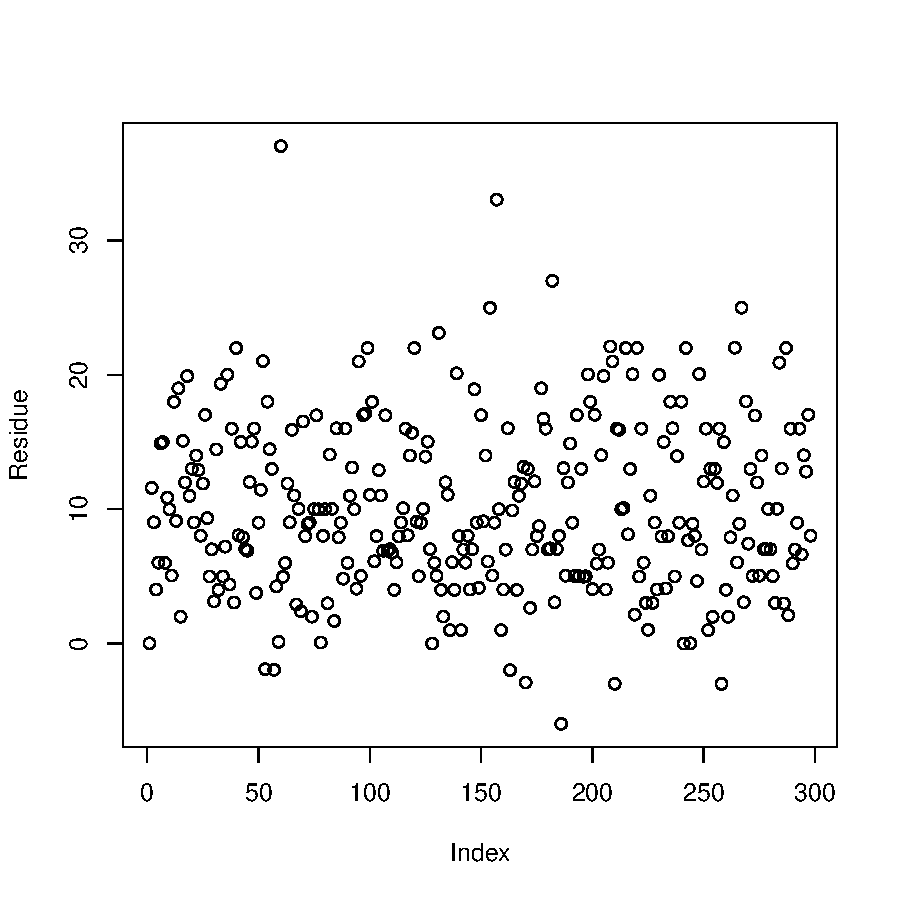
\includegraphics{Geyser-Analysis-log1_plot}
\hspace{1cm}
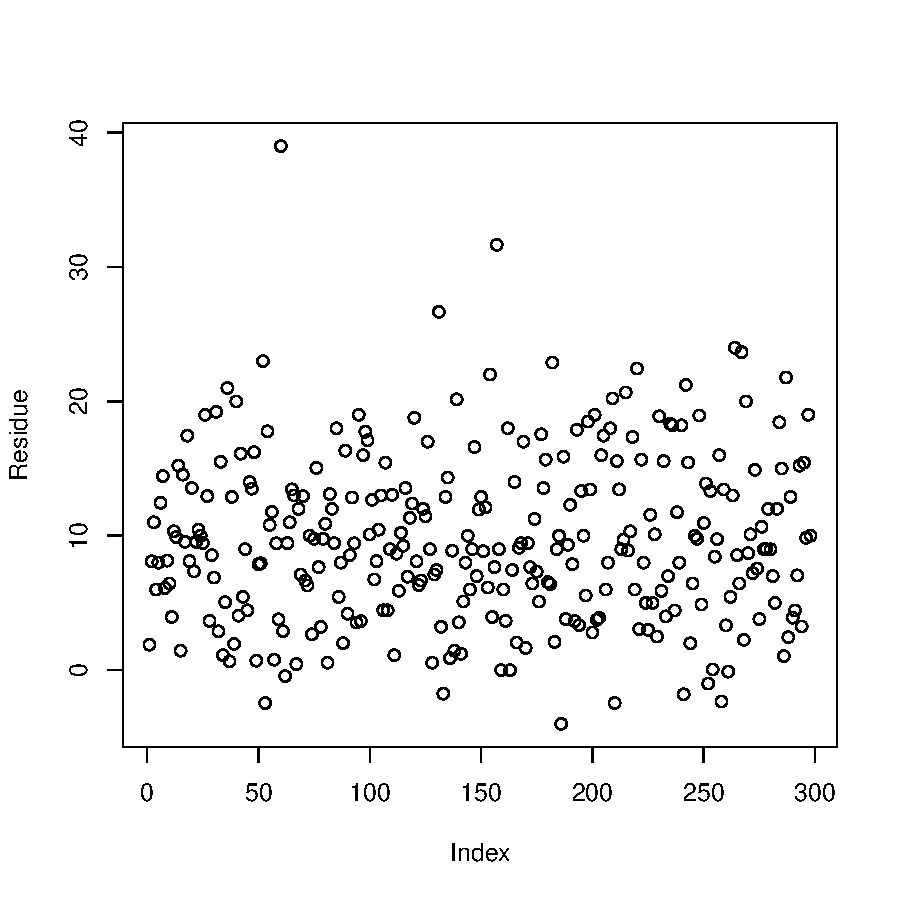
\includegraphics{Geyser-Analysis-plm1_plot}
\caption{Residuals of Model 1 (left) and Model 2 (right)}
\label{fig:residue1}
\end{figure}

\subsection{Linear model with predictors: duration \& waiting time}

This model is a slight adaption of the official predictive model, too. Instead of taking the clustering into account we add the last waiting time as a regressor. This leads to the following implementation:

\begin{Schunk}
\begin{Sinput}
> lm1.durwait <- function(x,p) {
+   d <- x$d
+   w <- x$w
+   p[1] + p[2]*d + p[3]*w
+ }
\end{Sinput}
\end{Schunk}

Because of the close relation to the park model, we use its parameters as inital parameters. For the waiting time coefficient we use 0 as we suspect it will only act as a small correction. The results can be found in Table~\ref{tab:lm1} and the residues are depicted in Figure~\ref{fig:residue2} on page~\pageref{fig:residue2}. As before, there is almost no structure in the residues, except for the known outliers.

\begin{table}[htbp]
\centering
\sisetup{
  table-number-alignment = right,
  table-format = -2.2
}
\begin{tabular}{r
S[table-auto-round]
S[table-auto-round]
S[table-auto-round]}
\toprule
& {Param1} & {Param2} & {Param3} \\
\midrule
Initial & 30 & 10
  & 0\\
Terminal & 30.49 & 10.02
  & -0.05\\
\bottomrule
\end{tabular}
\caption{Parameters of the linear (dur+wait) model}
\label{tab:lm1}
\end{table}

\subsection{Piecewise linear model with predictors: duration \& waiting time}

This model is a refinement of the previous one. Again we use duration and waiting time as predictors, yet this time we apply a linear model to each of the three identified clusters separately. This increases the number of parameters to 9 and the code takes the following form:

\begin{Schunk}
\begin{Sinput}
> plm2.durwait <- function(x,p) {
+   d <- x$d
+   w <- x$w
+   result <- c()
+   for(i in 1:length(d)) {
+     r <- 0
+     if(d[i] <= dsep) {
+       r <- p[1] + p[2]*d + p[3]*w
+     } else {
+       if(w[i] <= wsep) {
+         r <- p[4] + p[5]*d + p[6]*w
+       } else {
+         r <- p[7] + p[8]*d + p[9]*w
+       }
+     }
+     result <- append(x = result, values = r)
+   }
+   result
+ }
\end{Sinput}
\end{Schunk}

Because of the close relation to the park model. We use its parameters as inital parameters. For the different waiting times we use 0, as we suspect only a small corrective effect. The result is summarized in Table~\ref{tab:plm2} and the residues can be found in Figure~\ref{fig:residue2} (right). In this case there is a little more structure than in the other cases and we have the same outliers. Additionally we see that we miss more eruptions than in the other models. Together with the high number of necessary parameters, these are indicators against the use of this model.

\begin{table}[htbp]
\centering
\sisetup{
  table-number-alignment = right,
  table-format = -2.2
}
\begin{tabular}{r
S[table-auto-round]
S[table-auto-round]
S[table-auto-round]
S[table-auto-round]}
\toprule
& {Param1} & {Param2} & {Param3} & {Param4}\\ 
\midrule
Initial & 30 & 10
  & 0 & 30\\
Terminal & 29.98 & 10.11
  & -0.03 & 32.68\\
\bottomrule
\end{tabular}
\vphantom{h}
\vspace{0.3cm}
\vphantom{h}
\begin{tabular}{S[table-auto-round]
S[table-auto-round]
S[table-auto-round]
S[table-auto-round]
S[table-auto-round]}
\toprule
{Param5} & {Param6} & {Param7} & {Param8} & {Param9}\\
\midrule
10 & 0
  & 30 & 10
  & 0\\
  10.11 & -0.01
  & 30.01 & 9.88
  & -0.04\\
\bottomrule
\end{tabular}
\caption{Parameters of the piecwise linear (dur+wait) model}
\label{tab:plm2}
\end{table}

\begin{figure}[htbp]
\setkeys{Gin}{width=0.45\textwidth}
\centering
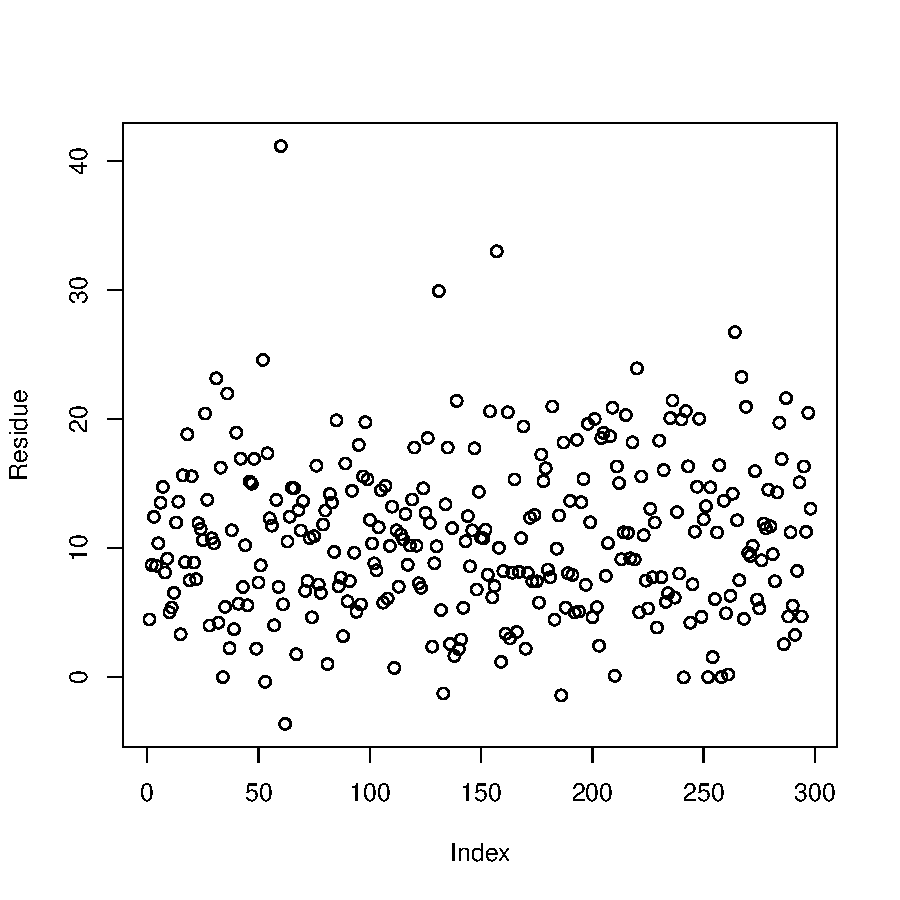
\includegraphics{Geyser-Analysis-lm1_plot}
\hspace{1cm}
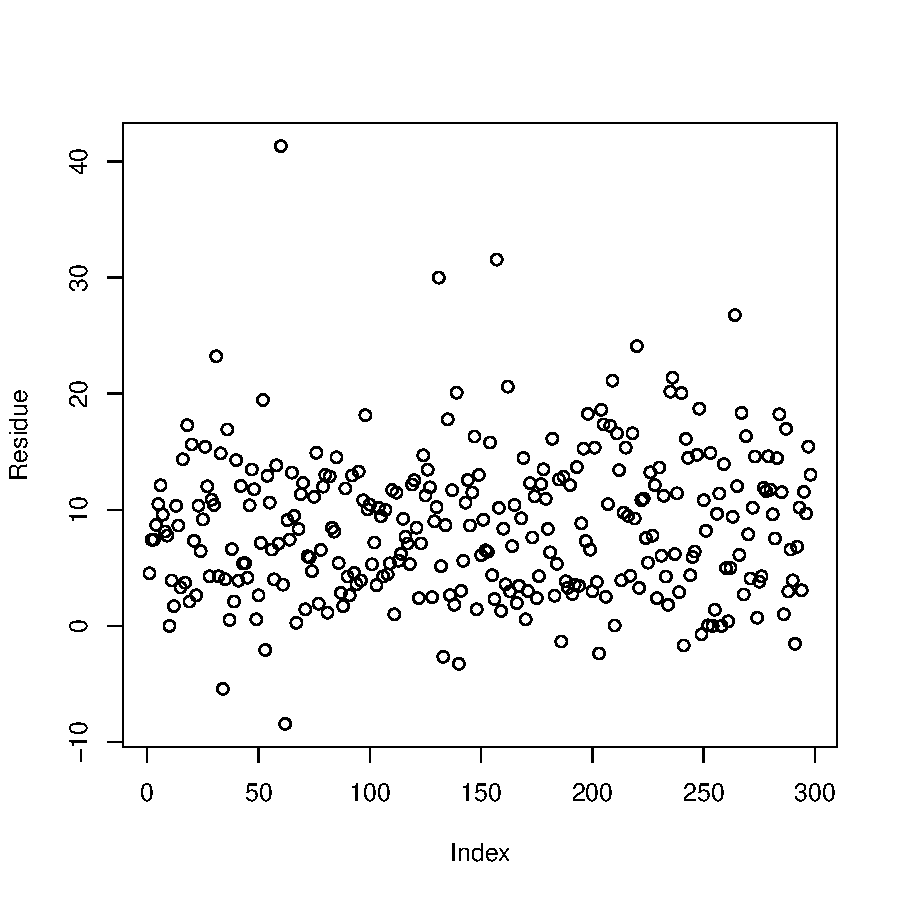
\includegraphics{Geyser-Analysis-plm2_plot}
\caption{Residuals of Model 3 (left) and Model 4 (right)}
\label{fig:residue2}
\end{figure}

\printbibliography[heading=bibintoc]

\end{document}
